%%%%%%%%%%%%%%%%%%%%%%% file template.tex %%%%%%%%%%%%%%%%%%%%%%%%%
%
% This is a general template file for the LaTeX package SVJour3
% for Springer journals.          Springer Heidelberg 2010/09/16
%
% Copy it to a new file with a new name and use it as the basis
% for your article. Delete % signs as needed.
%
% This template includes a few options for different layouts and
% content for various journals. Please consult a previous issue of
% your journal as needed.
%
%%%%%%%%%%%%%%%%%%%%%%%%%%%%%%%%%%%%%%%%%%%%%%%%%%%%%%%%%%%%%%%%%%%
%
% First comes an example EPS file -- just ignore it and
% proceed on the \documentclass line
% your LaTeX will extract the file if required
\begin{filecontents*}{example.eps}
%!PS-Adobe-3.0 EPSF-3.0
%%BoundingBox: 19 19 221 221
%%CreationDate: Mon Sep 29 1997
%%Creator: programmed by hand (JK)
%%EndComments
gsave
newpath
  20 20 moveto
  20 220 lineto
  220 220 lineto
  220 20 lineto
closepath
2 setlinewidth
gsave
  .4 setgray fill
grestore
stroke
grestore
\end{filecontents*}
%
\RequirePackage{fix-cm}
%
%\documentclass{svjour3}                     % onecolumn (standard format)
%\documentclass[smallcondensed]{svjour3}     % onecolumn (ditto)
\documentclass[smallextended]{svjour3}       % onecolumn (second format)
%\documentclass[twocolumn]{svjour3}          % twocolumn
%
\smartqed  % flush right qed marks, e.g. at end of proof
%
\usepackage{graphicx}
\usepackage{amsmath}
%
% \usepackage{mathptmx}      % use Times fonts if available on your TeX system
%
% insert here the call for the packages your document requires
%\usepackage{latexsym}
% etc.
%
% please place your own definitions here and don't use \def but
% \newcommand{}{}
%
% Insert the name of "your journal" with
% \journalname{myjournal}
%
\begin{document}

\title{PotteryVR: a Realtime Virtual Pottery Tool%\thanks{Grants or other notes
%about the article that should go on the front page should be
%placed here. General acknowledgments should be placed at the end of the article.}
}
%\subtitle{Do you have a subtitle?\cite{Jacob2008Reality}  \\ If so, write it here \cite{website:unity3d}}

%\titlerunning{Short form of title}        % if too long for running head

\author{Zihan Gao         %\and
        %Guangsheng Feng %etc.
}

%\authorrunning{Short form of author list} % if too long for running head

\institute{F. Author \at
              first address \\
              Tel.: +123-45-678910\\
              Fax: +123-45-678910\\
              \email{fauthor@example.com}           %  \\
%             \emph{Present address:} of F. Author  %  if needed
           \and
           S. Author \at
              second address
}

\date{Received: date / Accepted: date}
% The correct dates will be entered by the editor


\maketitle

\begin{abstract}
We present PotteryVR, an interactive virtual reality (VR) modeling system that allows novice users to create virtual pottery works with their bimanual movement using hand-held motion controllers.
Our system consists of two major components: a mesh generator and an interactive pottery model editor.
The mesh generator can procedurally generate a realistic clay mesh. With the interactive pottery model editor, the user can shape the clay mesh in realtime intuitively to create a virtual pottery work.
The virtual pottery created by our system can be exported as an obj file and used for 3D printing.
The results of our user study have shown that our system is easier to use compared with traditional modeling systems. Users without real life pottery making experience and 3D modeling knowledge can easily create pottery works with our system.


Insert your abstract here. Include keywords, PACS and mathematical
subject classification numbers as needed.
\keywords{First keyword \and Second keyword \and More}
% \PACS{PACS code1 \and PACS code2 \and more}
% \subclass{MSC code1 \and MSC code2 \and more}
\end{abstract}

%%% Introduction

\section{Introduction}
\label{sec:1}
%[CAD tools - hard to use]
Pottery is one of the oldest inventions in heterogeneous civilizations in human history for thousands of years, 
In recent years, emerging technologies such as 3D printing introduces a new way of pottery design, enabling people to fabricate pots in a digital manner with the help of Computer Aided Design (CAD) software and 3D printers.
There are several desktop CAD systems either from academic or industry, some of them are developed specifically for pottery design[a, b], which can generate 3D meshes based on the values from user keyboard and mouse input.
However, for novice users who are not professional 3D artists, these systems are formidable to learn due to complex user interfaces. 
This kind of systems limits the creativity of novice users, since it is quite challenging for them to master the tool in a short period of time.
In addition, the experience of creating potteries using CAD tools is far different from in reality.

%[in-air interaction system - freehand, lacks robustness, feedback and reality]
Traditional CAD tools, such as Maya[] and 3ds Max[], are formidable to learn due to complex user interfaces.
To address this situation, some camera-based virtual pottery systems such as [a, b, c] have been developed, which provides much simpler user interfaces, allowing users to design pots using freehand.
These works indeed provide a gentle learning curve, however, they have some common limitations.
First, freehand interactions from depth cameras lacks robustness due to jittering, whose inaccuracy hinders user experience severely.
Second, freehand interaction lacks haptic feedback, making it difficult for users to perceive if they have touched anything in VR environments.
In addition, some features of clay, namely shape irregularity, thickness etc., are missing from these systems, undermining realistic look and feel in the pot design process.

%[design goals: 1. simple 2. robust/realistic]
In this paper, we present PotteryVR, a VR system that allows users to design virtual pottery models from their hand movement using hand-held motion controllers. There are two major design goals for PotteryVR:
%[easy]
1 Provide a simple and intuitive interface for novice users to learn virtual pottery skills with minimum cognitive load.
%[robust realistic]
2 Design a robust virtual pottery system on VR devices that can generate realistic clay meshes and provide refined haptic feedbacks based on bimanual spatial interactions.

%[design considerations: 1.HCD 2. RBI]
Oviatt \cite{oviatt2006human} concluded that human-centered design can minimize users’ cognitive load, which effectively frees up mental resources for performing better while also remaining more attuned to the world around them.
%% TODO
So we take the human-centered design approach, which models users’ natural behavior to begin with so that interfaces can be designed that are more intuitive, easier to learn, and freer of performance errors.
In addition, Jacob et al. \cite{Jacob2008Reality} summarized that the designer's goal should be to allow the user to perform realistic tasks realistically, to provide additional non real-world functionality, and to use analogies for these commands whenever possible.
Hence, while we design our system based on pottery creation process in reality to minimize the effort, we should provide convenient functionality in our system for efficiency.

%[contributions]
The main contributions of our works are:

1 Present a virtual pottery system which can generate pot models from user spatial interaction for 3D printing.

2 Propose a virtual pottery workflow by introducing simple and intuitive user interfaces for modeling, enabling novice users to understand and learn pottery production pipeline.

3 Conduct an user study showing the comparison results among three interaction systems. The results have shown that our system is easier to use compared with traditional 3D modeling tools and is more intuitive and immersive than touchscreen based interfaces.

%%%

\section{Related Work}
\label{sec:2}

\subsection{Bimanual Interaction}
\label{sec:2.1}
Bimanual interaction has been a popular research field, which can accomplish a variety of tasks in both physical and virtual environments.
In terms of mechanisms, bimanual interaction can be classified into two categories: bare-hand based interactions and instrument based interactions.

There are a great number of research efforts \cite{walter2014cuenesics,cui2016exploration,ramani2015gesture,murugappan2013handy,han2014virtual} on bare-hand based interactions using depth camera such as Kinect, Leap Motion etc.
Cuenestics \cite{walter2014cuenesics} is a design space for hand-gesture based mid-air selection techniques using a depth camera Kinect, where users can select contents on interactive public displays with their gesture input.
Cui et al. \cite{cui2016exploration} proposed a modeling system with natural free-hand interaction using a Leap Motion controller, allowing users to grab and manipulate objects with one or two hands intuitively.
While these works provided accessibility to users, the limitations are obvious as well: The input is not always accurate due to many factors such as lighting condition and occlusion, which might cause user frustration.
In addition, these methods do not provide haptic feedbacks, which hinders the realistic feel for users.

Unlike bare-hand based interactions, instrument based interactions provide more control precision, haptic feedback and unambiguity.
Surface Drawing \cite{schkolne2001surface} is a system for creating organic 3D shapes using tangible tools such as gloves, where users can define strokes with the path of hands wearing gloves.
Hinckley et al. \cite{hinckley1998two} did a research on two-handed virtual manipulation with a point design of a prop-based system, which allows users to view a cross section of a brain with interface props.
These works have a common problem that the usage of these instruments are limited to a lab context that very few users can access.
There are a number of motion controllers such as Wii Remote \cite{wingcrave2010wii} and HTC Vive \cite{niehorster2017accuracy} that become widely commercialized products and accessible to consumers, as well as used in scientific research.
In our project, HTC Vive system is used in our system, which provides precision, haptic feedback and well accessed by consumers.

\subsection{Artistic Tools in VR}
\label{sec:2.2}
Virtual Reality has shown great potential for art and design, which not only provides immersive and intuitive interfaces for user, but also creates new art medium, new art form and novel experience\cite{laviola20113d}. CavePainting \cite{keefe2001cavepainting} is a 3D artistic medium in a fully immersive environment, which enables artists to create spatial paintings with physical props and gestures. Agrawala et al.\cite{agrawala19953d} developed an interface for painting on polygon meshes using a 6DOF space tracker, which provides a natural force-feedback for painting, allowing users to place colors on meshes intuitively. MAI Painting Brush++ \cite{otsuki2017brush} is a brush device for virtual painting of 3D virtual objects, where users could take a physical object in the real world and apply virtual paint to it with visual and haptic feedback. Virtual Clay \cite{mcdonnell2001virtual} is a sculpture framework based on subdivision solids and physics-based modeling, which is equipped with natural, haptic based interaction, providing users with a realistic sculpting experience. Sheng et al. \cite{sheng2006interface} proposed an interface for virtual 3D sculpting, which uses camera-based motion tracking technology to track passive markers on the fingers and prop, enabling users to apply operations such as deforming, smoothing, pasting and extruding.

\subsection{Virtual Pottery Systems}
\label{sec:2.3}


Several systems have been developed for virtual pottery, unlike other sculpting systems mentioned above, v
Qp \cite{koutsoudis2009qp} was a tool for generating 3D pottery models, which can produce a collection of random 3D ancient greek vessels.
Based on number-theoretic techniques, Kumar et al. \cite{kumar2011wheel} presented a system for creating digital potteries including thick-walled potteries as well, which resembles pottery works in real life.
While these systems can generate heterogeneous pottery models efficiently, their user interfaces are limited to traditional keyboard and mouse input, which are not helpful for users to understand the pottery creation process.
%%CHINA korida1997interactive
Handy-Potter \cite{murugappan2013handy} was a rapid 3D creation tool, which tracks user skeletons with depth sensing camera Kinect, enabling users to create potteries using hands and arms.
%%CAD ramani2015gesture
Han et al. \cite{han2014virtual} presented an audiovisual interface, where hand motions are translated into musical sound.
In AR Pottery \cite{han2007ar}, augmented reality has been applied to pottery design, with which users can deform a virtual pottery using a marker held by hand.
Although with these systems users could create some virtual pottery works, the actions applied are quite different from real life pottery making process. Thus, users cannot learn the actual pottery process from using these systems.

[design consideration - EDUCATION!!!]
In contrast to existing works, our system provides a novel pottery creation workflow in virtual reality which lets user shape and color pottery through two-handed spatial interactions, helping novice users to understand and learn real life pottery.



\section{Workflow}
\label{sec:3}

The pottery creation process on a pottery wheel is called "throwing", where a ball of clay is placed in the centre of a turntable, called the wheel-head, which the potter rotates with a stick, with foot power or with a variable-speed electric motor.
To illustrate the pipeline of pottery creation in our system, an example workflow using PotteryVR is described as follows.

When a user starts to use PotteryVR, a realistic clay mesh is automatically generated with Perlin noise. (Figure 2a, Section 4.1)
Similar to the pottery operation in reality, the user first need to use both hand to make the irregular clay shape into perfect rotational symmetry, which is called \textit{centring}. (Figure 2b, Section 4.2)
In order to control the thickness of the clay (i.e. \textit{opening}), the user need to press down the clay to create a hollow in the clay. (Figure 2c, Section 4.3)
Then the user can draw up the walls (i.e. \textit{pulling}) with two hands moving up together, controlling the height of the clay. (Figure 2d, Section 4.4)
The system supports mesh deformation (\textit{throwing}) and smoothing, where the user can adjust related parameters to get ideal pot.
After the creation is done, the user can save the screenshot and save the pottery model as an OBJ file, which can be used for 3D printing.
% For one-column wide figures use
\begin{figure}
% Use the relevant command to insert your figure file.
% For example, with the graphicx package use
  
\includegraphics{example.eps}
% figure caption is below the figure
\caption{Please write your figure caption here}
\label{fig:1}       % Give a unique label
\end{figure}


\section{Implementation}
\label{sec:4}

In this section, we will describe more details about the implementation. 



\subsection{Mesh Generation}
\label{sec:4.1}

Most of Virtual Pottery systems approximate the initial shape of pottery clay as a primitive cylinder shape[a, b, c]. While this approach is simple to implement, it ignores subtle details of clay in real life, whose irregularity needs to deal with during the creation process. Unlike the existing systems, we approximate the initial shape of the clay on the pottery wheel as a blend of cylinder and semi-ellipsoid, then adding Perlin noises to mimic the clay in reality.

%Cylindrical coordinate system

\paragraph{Basic clay} We describe the clay mesh as a series of circular sections in different heights, whose resolution can be defined by radial sections $s_{r}$ and vertical sections $s_{v}$. Given radius $r$ and height $h$, our system can generate primitive mesh of cylinder and semi-ellipsoid respectively (Fig 1a, 1b).
For each vertex in the mesh, we use a $m \times n$ matrix $M$ to store radius values, where number of row $m = s_{v} + 1$ and the number of column $n = s_{r}$ respectively. The base radius $r_{base_{i}}$ of each vertex $\mathbf{v}_{ij}$ in row $i$ can be written as: 
\begin{equation}
\begin{split}
r_{base_{i}} = \alpha \cdot \frac{r}{h} \sqrt{h^2 -  h_{i}^2} + (1 - \alpha) \cdot r \\
h_{i} = i \cdot \frac{h}{m-1}
\end{split}
\end{equation}
where $\alpha$ is a factor controls the shape blending between a  cylinder (when $\alpha=0$) and a semi-ellipsoid (when $\alpha=1$) (Fig 2).
While the shape of clay can be roughly approximated like this, in real life the actual clay shape is not regular, whose irregular features needs to be handled during the pottery creation process.

\begin{figure*}
% Use the relevant command to insert your figure file.
% For example, with the graphicx package use
  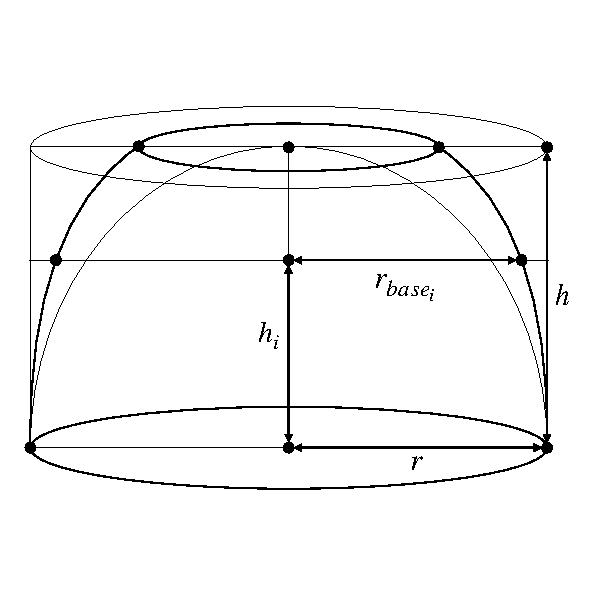
\includegraphics[width=0.75\textwidth]{f1.pdf}
% figure caption is below the figure
\caption{Please write your figure caption here}
\label{fig:1}       % Give a unique label
\end{figure*}

\paragraph{Adding noise} To address this issue, we add some randomness to the vertices to mimic the realistic clay using Perlin Noise [..], which is a smooth random method proposed by Ken Perlin in 1985. We randomize the centre and radius for each circle, then add noise to individual vertices.
To add noise to the centre, we use random $\phi_{i} \in [0, 2\pi]$ and $r_{c_{i}}$ to present the centre
$\mathbf{O}_{i} = \left[r_{c_{i}}cos\phi_{i}, 0, r_{c_{i}}sin\phi_{i}\right]^T$
. Then we sum the values for each radius
$r_{total_{i,j}} = r_{base_{i}} + r_{row_{i}} + r_{indv_{i,j}}$
, where $r_{row_{i}}$ is the radius for each circle, and $r_{indv_{i,j}}$ is individual radius for each vertex.(Fig 3) We can get the radius value $r_{i,j}$ in the matrix $M$ for each vertex, and calculate the vertex position $\mathbf{v}_{ij}$ based on the radius values in the matrix:
\begin{equation}
\begin{split}
r_{i,j} = \left\|
\mathbf{O}_{i} + \left[ r_{total_{i,j}} cos \theta_{j},
h_{i},
r_{total_{i,j}} sin \theta_{j}
\right]^T
\right\| \\
\mathbf{v}_{i,j} =
\left[r_{i,j}  cos \theta_{j},
h_{i},
r_{i,j} sin \theta_{j}\right]^T \\
\theta_{j} = j \cdot \frac{2\pi}{n}
\end{split}
\end{equation}

\begin{figure*}
% Use the relevant command to insert your figure file.
% For example, with the graphicx package use
  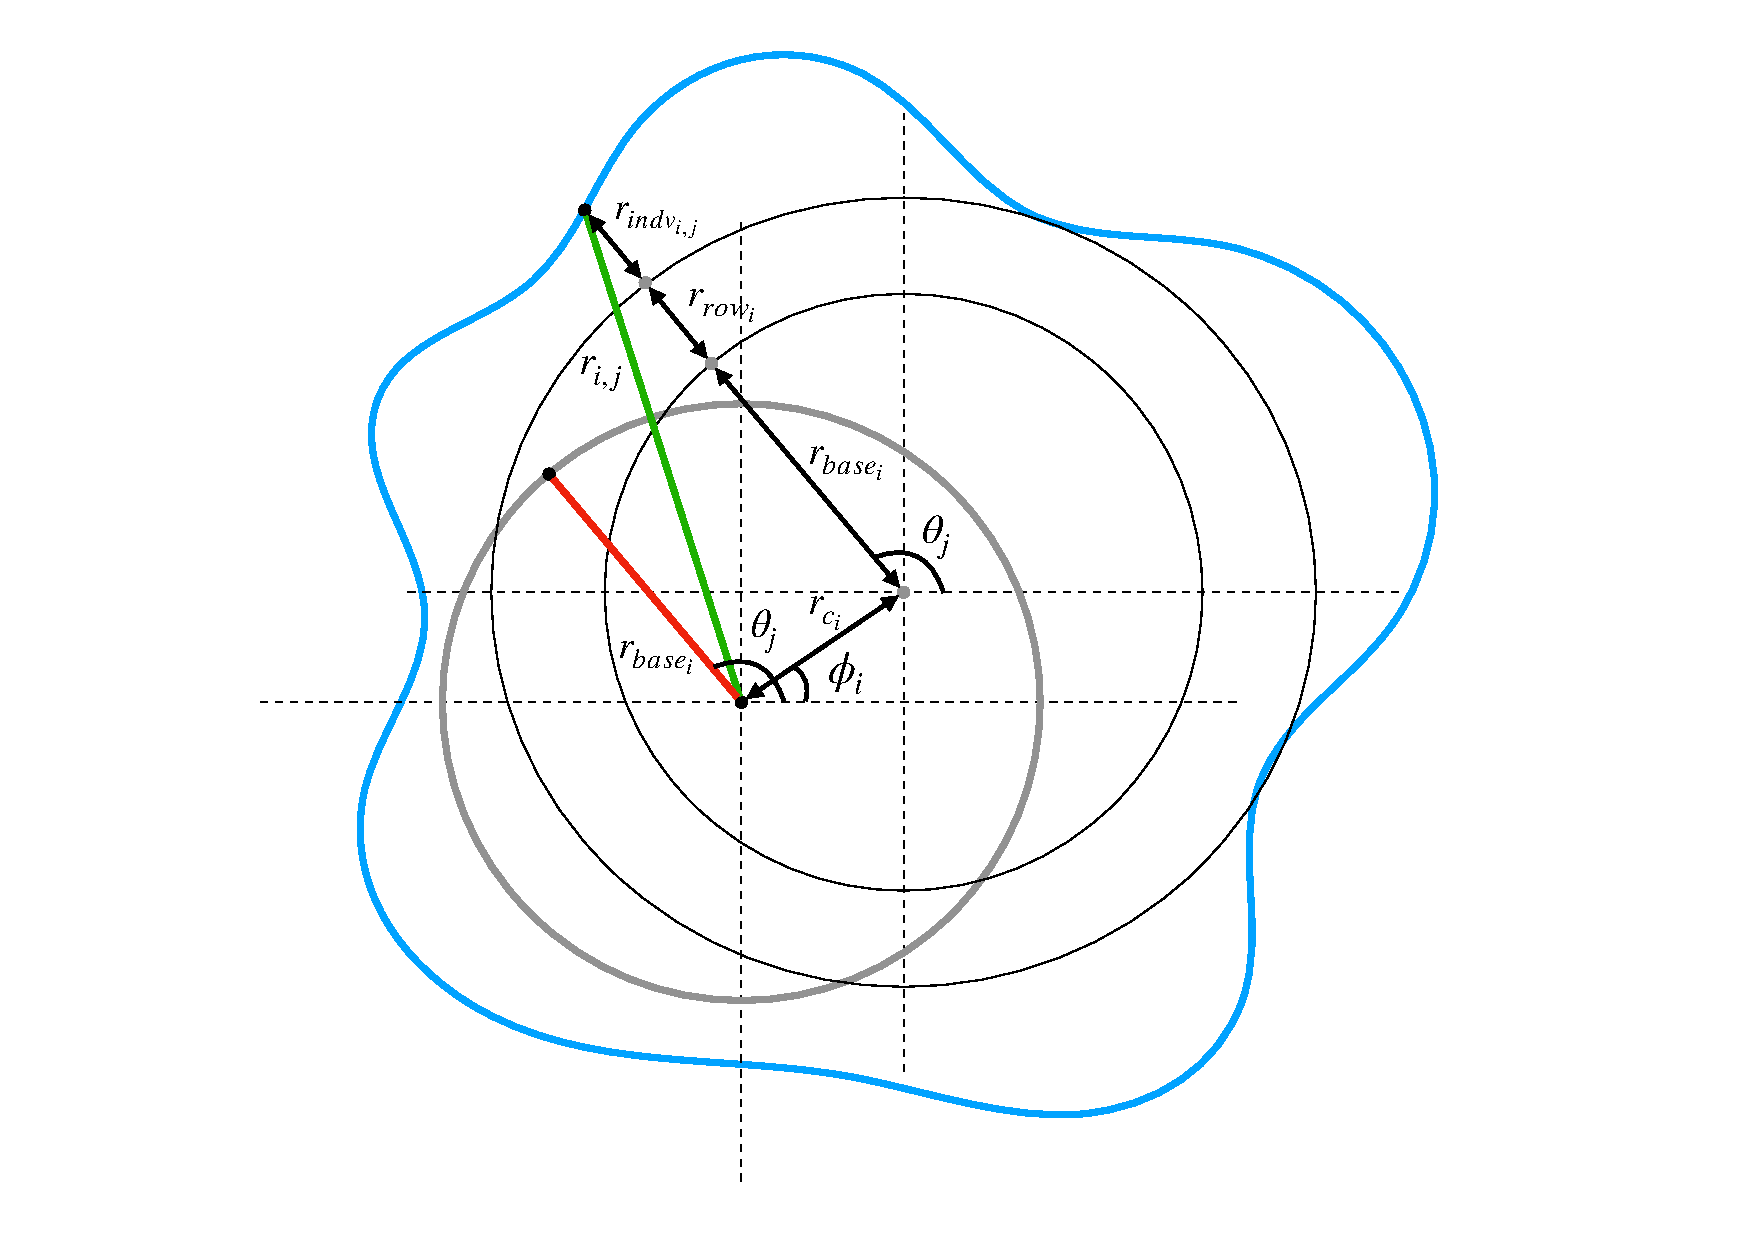
\includegraphics[width=0.75\textwidth]{f2.pdf}
% figure caption is below the figure
\caption{Please write your figure caption here}
\label{fig:1}       % Give a unique label
\end{figure*}

Unlike other virtual pottery creation system, we aim to create 3D printing oriented pottery models. To accomplish that we need to generate watertight 3D models. Hence, our system generate inner and bottom sides based on the outer side mesh. The vertices on inner side can be denoted as:
\begin{equation}
\begin{split}
\mathbf{v'}_{i,j} = 
\begin{bmatrix}
1 - \beta & 0 & 0 \\
0 & 1 & 0 \\ 
0 & 0 & 1 - \beta 
\end{bmatrix}
\mathbf{v}_{i,j}
\end{split}
\end{equation}
where $\beta$ is the thickness value of the clay mesh. In mesh generation phase, the initial value of $\beta$ is 1; in mesh deformation phase, the value of $\beta$ can be adjusted by user.
We then generate vertices for both inner-bottom and outer-bottom sides according to inner-side and outer-side vertices respectively. Finally, a mesh can be generated by constructing triangle faces based on the vertex indices. (Fig)


\subsection{Mesh Editing}
\label{sec:4.2}
After observing and analyzing several real life pottery-making videos, we put mesh editing operation into 3 categories: height/thickness control, mesh deformation and mesh smoothing. These operations will be discussed in detail in the following sections.

//deformation strategy: modify the feature variables, then update the mesh in realtime

\subsubsection{Symmetric Control}
\label{sec:4.2.1}
In real life, clay on pottery wheel can swing around vertical axis due to asymmetry. 

// so, radial smoothing is needed to make the clay symmetric.(Fig)
In our implementation, average radius for each row is calculated and each radius in matrix  needs updated:
\begin{equation}
\begin{split}
r'_{i,j} = 
\lambda \cdot \frac{1}{n}\sum_{k=1}^{n} r_{i,k}
+ (1 - \lambda) \cdot r_{i,j}
\end{split}
\end{equation}
where $\lambda \in [0,1]$ is a damping factor controlling the radial smoothing effect.

% For one-column wide figures use
\begin{figure}
% Use the relevant command to insert your figure file.
% For example, with the graphicx package use
  
\includegraphics{example.eps}
% figure caption is below the figure
\caption{Please write your figure caption here}
\label{fig:1}       % Give a unique label
\end{figure}

\subsubsection{Thickness/Height Control}
\label{sec:4.2.2}
Height and thickness control are  basic clay manipulations in pottery creation process which are done by applying force to clay with two hands. The height can be adjusted by hands vertical movement while holding the clay, while the thickness can be adjusted by pushing down the top centre part of the clay with fingers. Let  be the vertical hand movement distance, we have:
\begin{equation}
\begin{split}
\Delta y = (\Delta y_{l} + \Delta y_{r})/2 \\
h' = h_{0} + \Delta y * \gamma \\
\beta' = \beta_{0} + \Delta y/ h
\end{split}
\end{equation}
where $h_{0}$ and $\beta_{0}$ are previous height and thickness values before every deformation respectively; $\gamma$ is a damping factor for height.

% For one-column wide figures use
\begin{figure}
% Use the relevant command to insert your figure file.
% For example, with the graphicx package use
  
\includegraphics{example.eps}
% figure caption is below the figure
\caption{Please write your figure caption here}
\label{fig:1}       % Give a unique label
\end{figure}

\subsubsection{Mesh Deformation}
\label{sec:4.2.3}
In this section we talk about interactively deforming. This topic is challenging since complex mathematical formulations (1) have to be hidden behind an intuitive user interface and (2) have to be implemented in a sufficiently efficient and robust manner to allow for interactive applications.[Polygon Mesh Processing] 

a set of handle points
fixed points
due to rotational symmetry in pottery vessels, the deformation problem is turned into how to get the new radius Matrix

We calculate weights based on hand initial position p0 [FIG]
\begin{equation}
\begin{split}
r'_{ij} = r_{ij} + s \cdot l \cdot w_{ij} \\
d(r_{i,j}) = \begin{cases}
\rho' - \rho_{0} &  d < r_{i} \\
0 &  d > r_{o} \\
s(\frac{d}{r_{o}-r_{i}}) (\rho' - \rho_{0}) &  r_{i} < d < r_{o}
\end{cases}
\end{split}
\end{equation}
where $d$ is the vertical distance between the handle and $\mathbf{v}_{i,j}$; $r_{i}$ and $r_{o}$ are inner and outer handle radius respectively. 

(ρ, φ, z) 
The radial distance ρ is the Euclidean distance from the z-axis to the point P.
The azimuth φ is the angle between the reference direction on the chosen plane and the line from the origin to the projection of P on the plane.
The height z is the signed distance from the chosen plane to the point P.

\begin{figure*}
% Use the relevant command to insert your figure file.
% For example, with the graphicx package use
  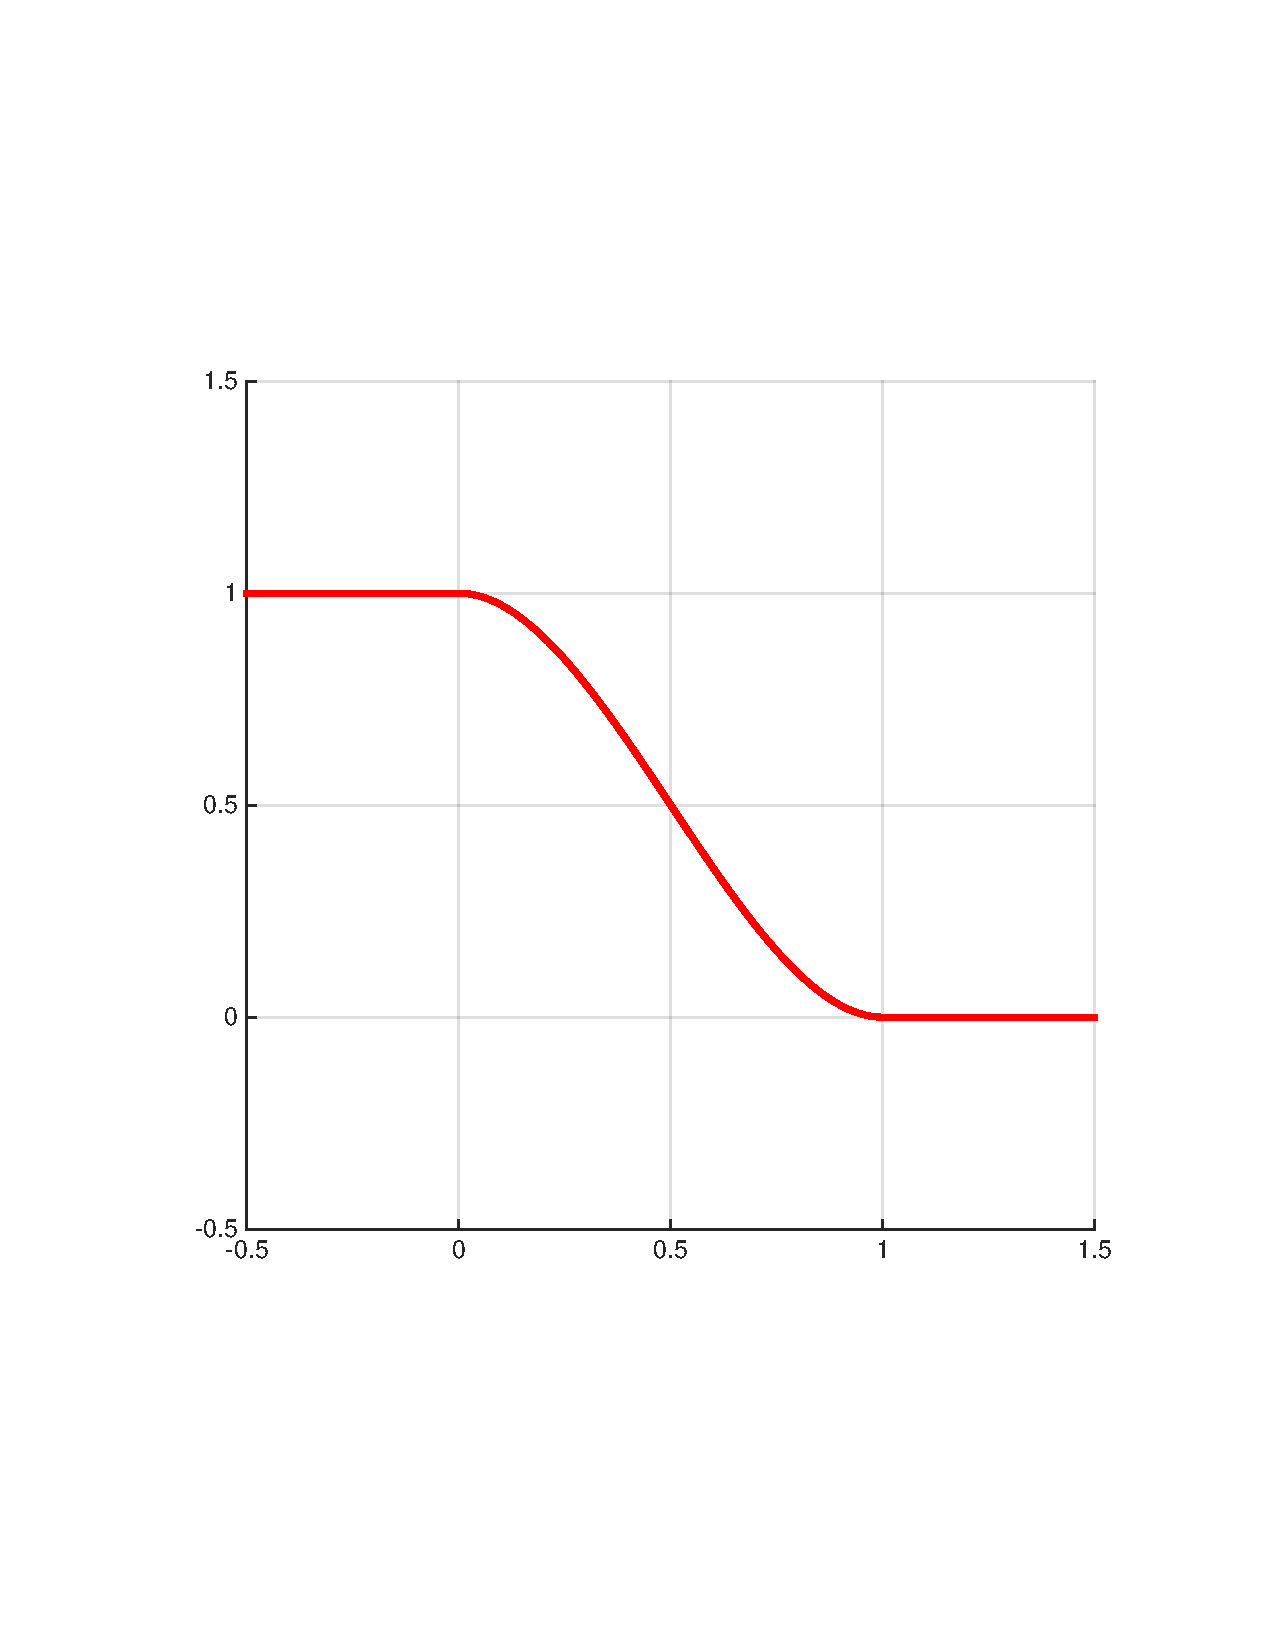
\includegraphics[width=0.75\textwidth]{f4.pdf}
% figure caption is below the figure
\caption{Please write your figure caption here}
\label{fig:1}       % Give a unique label
\end{figure*}

\subsubsection{Mesh Smoothing}
\label{sec:4.2.4}
As mentioned above, it is possible to create sharp features upon the clay mesh when  is large. Hence, we use Laplacian smoothing in our system to smooth sharp features: 
\begin{equation}
\begin{split}
r'_{i,j} = 
\mu  \frac{1}{N} 
\sum_{k=1}^N r_{k}
+ (1 - \mu)  r_{i,j}
\end{split}
\end{equation}
where $N$ is the number of adjacent vertices of $\mathbf{v}_{i,j}$; $\mu \in [0,1]$ is a factor controlling the radial smoothing effect.

\subsection{Interactions}
\label{sec:4.3}

the system in a virtual studio - pottery wheel

In our implementation, we use HTC Vive headset and hand-held controllers (Fig) to track user movements and inputs.

The goal of our system is not only to provide realistic experience in pottery creation, but also to provide convenient operations to improve the efficiency of pottery design. 
[reality based interaction - superpowers]
As a result, our system offers several operations in VR to support the design.

[descriptions]
buttons on the side of the pottery wheel

There are three main operations supported by our system:

Undo/Redo
Our system provides  capturing the state of the program before user actions.

New Mesh

Export Mesh

Radius adjustment

\subsection{Haptic Feedback}
\label{sec:4.4}

on touch feedback

range of area

movement resistance


\section{Results}
\label{sec:5}
We have implemented DigiClay using Unity3D and HTC Vive virtual reality system. 
Based on the common size of clay placed on pottery wheels, we set the height 0.2 units with the radius 0.15 units. Moreover, we assign 60 and 59 to radial segments and vertical segments respectively, thus we get m = 60 and n = 10 as the resolution of the clay. The parameters for Perlin noise generation are listed in Table 1.
%[noise parameters]
% For tables use
\begin{table}
% table caption is above the table
\caption{Please write your table caption here}
\label{tab:1}       % Give a unique label
% For LaTeX tables use
\begin{tabular}{lll}
\hline\noalign{\smallskip}
name & value & meaning  \\
\noalign{\smallskip}\hline\noalign{\smallskip}
$s_{Center}$ & 0.1 & Noise Scale of Center Distance \\
$s_{Angle}$ & 0.1 & Noise Span of Center Angle \\
$s_{Radius}$ & 0.1 & Noise Scale of Radius \\
$s_{Radius}$ & 0.1 & Noise Span of Radius \\
$s_{Vertex}$ & 0.1 & Noise Scale of Individual Vertex \\
$s_{Vertex}$ & 0.1 & Noise Span of Individual Vertex \\
\noalign{\smallskip}\hline
\end{tabular}
\end{table}

[deform parameters]
We set the outer radius of handle 0.2 units, and the inner ratio of handle 0\% to get smooth deformation effect as the process begins. The centring parameter $\lambda$ and smoothing parameter $\mu$ are set 0.5 and 0.7 respectively to damping the deformation.

[performance]
m, n, vertices, faces

\begin{table}
% table caption is above the table
\caption{Please write your table caption here}
\label{tab:1}       % Give a unique label
% For LaTeX tables use
\begin{tabular}{llll}
\hline\noalign{\smallskip}
radius segment & vertical segment & vertex number & face number \\
\noalign{\smallskip}\hline\noalign{\smallskip}
100 & 100 & 10000 & 10000 \\
100 & 100 & 10000 & 10000 \\
100 & 100 & 10000 & 10000 \\
\noalign{\smallskip}\hline
\end{tabular}
\end{table}

\section{User Study}
\label{sec:6}
In order to compare our system with prior modeling systems and tablet apps, we set up a comparative user study. We chose Autodesk Maya[] as the representative of traditional desktop modeling systems and Let's Create Pottery as the representative of tablet pottery creation systems.

\subsection{Evaluated Systems}
\label{sec:6.1}
The three evaluated systems were as follows:

\paragraph{PotteryVR}: our interactive pottery creation tool on virtual reality systems. The user can shape the virtual clay with bimanual spatial interaction.
\paragraph{Let’s Create! Pottery}: a touch-based pottery creation tool on mobile devices. Users can interactively create pottery models by fingers swiping on screens.\cite{website:letspottery}
\paragraph{Autodesk Maya}: a traditional desktop modeling system, which provides a set of powerful tools for professional 3D artists. The user can edit vertex, edge, face etc with mouse and keyboard.

Although the three systems are different, we focus on comparing them based on their similarities and workflows.
To investigate the influence of modeling process, we compare DigiClay and Autodesk Maya since they both support 3D modeling. They differ in workflow to create a pottery mesh. While DigiClay can automatically generate a clay mesh for deformation with motion controllers, Maya needs to create the mesh from a primitive cylinder in order to edit in vertex mode, edge mode or face mode with mouse and keyboard. 


\subsection{Participants}
\label{sec:6.2}
15-20 participants were participated in our user study, 9 male and 10 female, whose age ranged from 22 to 40 years. 10 of the subjects are familiar with VR systems (50\%); 5 of the subjects have experience with 3D modeling tools (20\%); 8 of the subjects have amateur pottery throwing experience in real life.
Figure 11 shows two subjects using our system to throw pottery. Figure 12 shows more results created by the subjects.

\subsection{Experimental Design and Procedure}
\label{sec:6.3}

After a 15 min training of the three systems, each subject had to accomplish 3 tasks:

Task\textsubscript{DigiClay}

Task\textsubscript{LetsPottery}

Task\textsubscript{Maya}

[Task details]

%[NASA-TLX]
After accomplishing each task, the subjects were asked to answer a questionnaire with six questions to measure the six dimensions of NASA-TLX, which includes physical demand, mental demand, temporal demand, effort, performance and frustration. 5 additional questions were asked after they finished all tasks.

Questions

\paragraph{Q1} Which one do you prefer to use to design a pottery, Maya or DigiClay?
\paragraph{Q2} Which experience do you prefer, the touchscreen based Let's Create Pottery or virtual reality based DigiClay?
\paragraph{Q3} Rank the three systems according to their supports for your imagination and creativity from high to low.
\paragraph{Q4} Rank the three systems according to your preference from high to low.

%[Some explanations]
NASA-TLX has been chosen in our research because it is widely used in human factor studies which addressed questions about interface design and evaluation.[NASA-TLX] We selected NASA-TLX as a part of our questionnaire to assess user workload in the three systems. Since the functionalities are different among the three systems, it is impossible and unfair to compare the interactions. We intended to allow our subjects to experience those differences and similarities through these tasks and analyze which types of interactions and results were more attractive to them through our user study questions.





\subsection{Study Results}
\label{sec:6.4}

%[basic introduction]
Figure A shows mean values of the six dimensions of NASA-TLX for all the tasks. For the questions of ranking, we count a score of 3 for the system in the highest ranking and 1 for the system in the lowest ranking. Figure B shows the vote results of the last two of the additional questions. Figure C shows the percentages of the first ranking frequencies of the three systems in the last two additional questions, in other words, how many female/male gave the highest rankings to the system.
%[DC - less time and mental demand]
According to Figure A, we can get some findings. 
Firstly, the mental demand value of Tmaya (M = 9.9) is much higher than the values of Tdigi (M = 0.1) and Tlcp (M = 0.2). Similarly, the temporal demand value of Tmaya (M = 9.9) is much higher than the values of Tdigi (M = 0.1) and Tlcp (M = 0.2). This indicated that DigiClay was less time-consuming and easier to use than Maya and LCP.
%[DC - easy to use, natural interaction]
Compared with the formidable interfaces and the modeling operations heavily rely on mouse and keyboard in Maya, DigiClay provides simple interfaces with intuitive bimanual interactions to deform the mesh. In our experiments, we found that it is not difficult for the subjects to understand how to deform the mesh in DigiClay compared with the difficulties of selecting and editing vertices and faces in Maya. Since the natural interactions in DigiClay are closely related to the operations in reality, the subjects can learn our system with ease.
%[LCP - limitation] [thickness smooth sharpness]
We also found that it was not as easy as we predicted for the subjects to design potteries when using the Let's Create Pottery app. There are some limitations in the throwing process in LCP, where subjects cannot modify the thickness of the clay. Moreover, subjects found it is impossible to create sharp features on the clay in LCP. 
%[Maya - hard]
Maya showed much higher values in mental demand (M = 0.2), effort (M = 0.2) and frustration (M = 0.2) and lower value in performance (M = 0.2) compared with DigiClay and LCP. Although mouse and keyboard based interaction allows precise controls, many subjects struggled with selecting and manipulating vertices and faces accurately.
%[user preference][enjoyable and intuitive]
The results also showed that a majority subjects preferred the experience of designing pottery in DigiClay than those of Maya, as shown in Figure C. In addition, more than 50\% subjects considered DigiClay stimulate their creativity the most and chose it as their favorite system among the three systems. From their feedbacks, we found that immersive interactions in virtual reality context gave them a novel and realistic way to interact with virtual pottery models when using DigiClay.
%[sex preference difference]
\begin{figure*}
% Use the relevant command to insert your figure file.
% For example, with the graphicx package use
  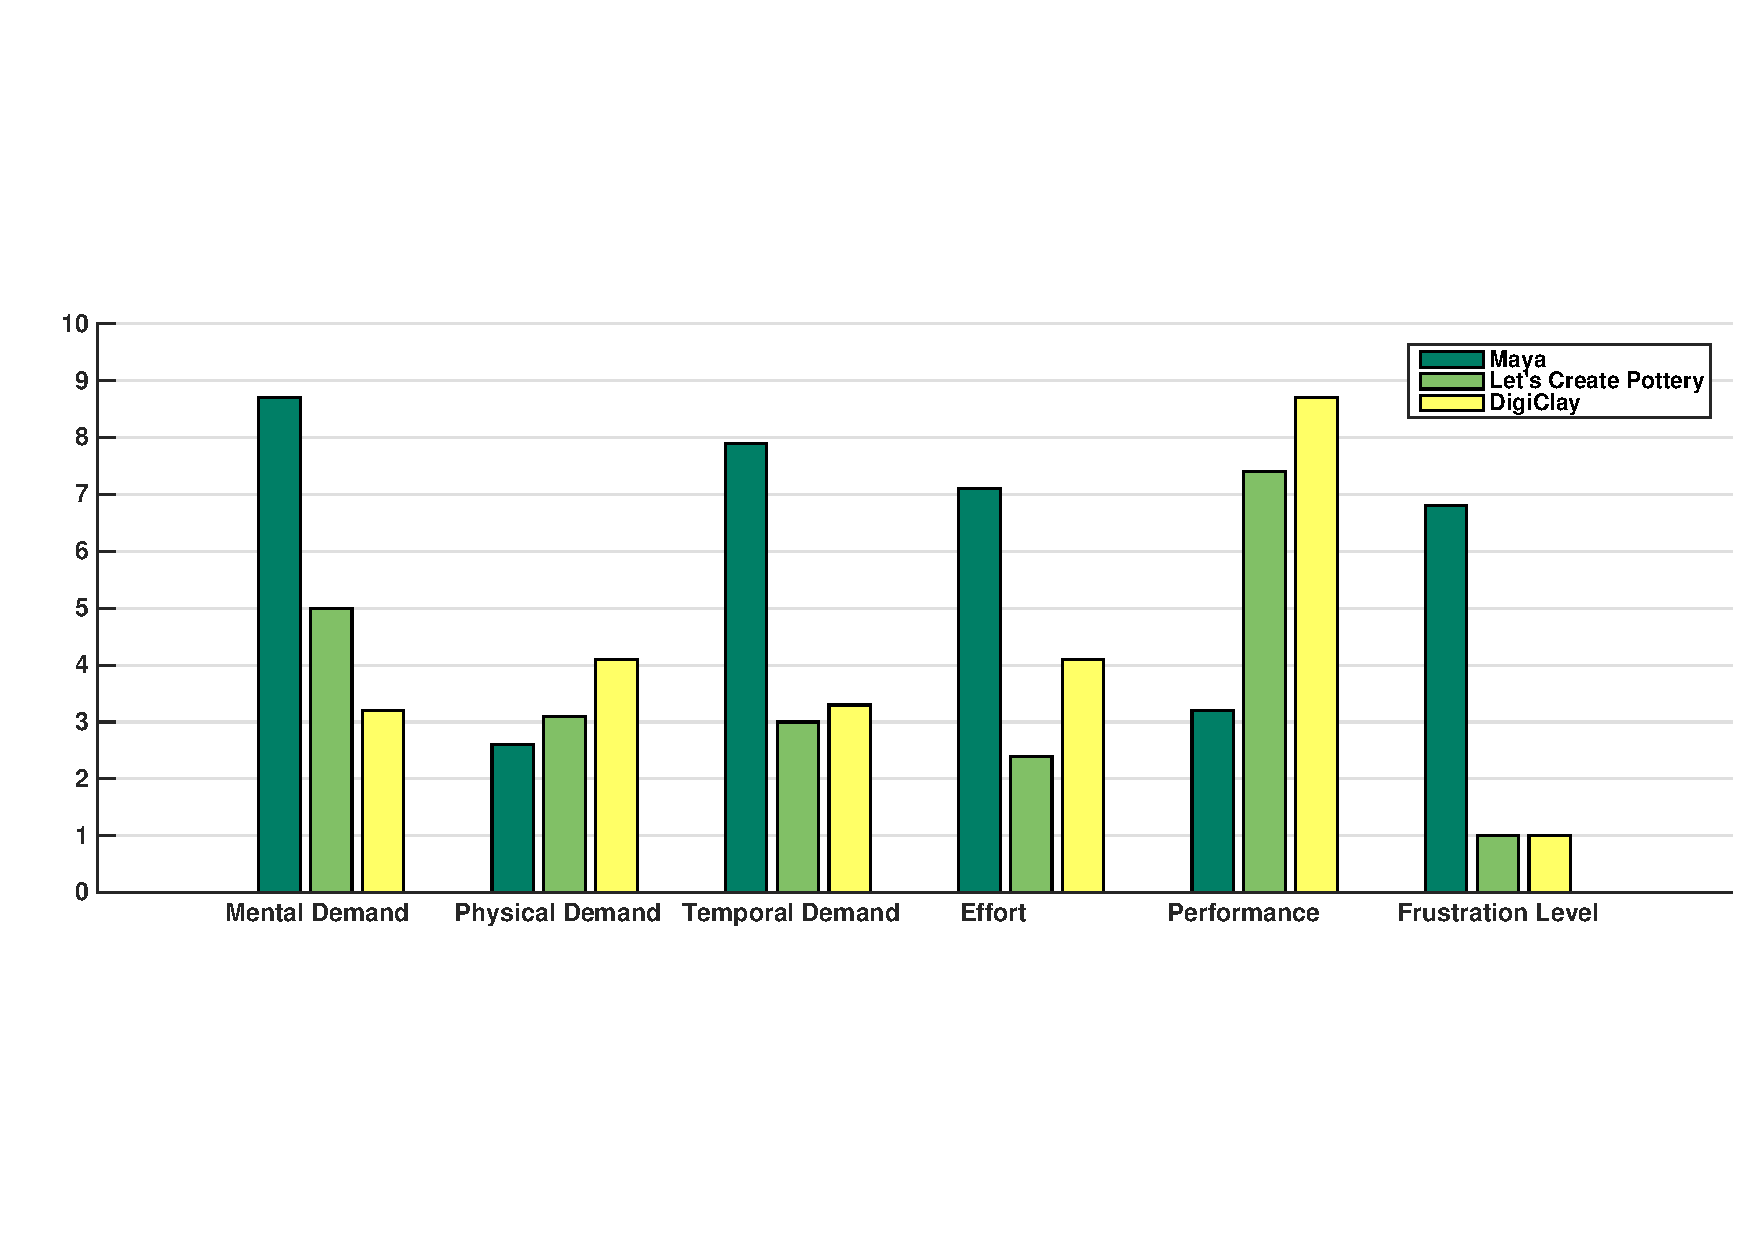
\includegraphics[width=0.75\textwidth]{f7.pdf}
% figure caption is below the figure
\caption{Please write your figure caption here}
\label{fig:1}       % Give a unique label
\end{figure*}

\begin{figure*}
% Use the relevant command to insert your figure file.
% For example, with the graphicx package use
  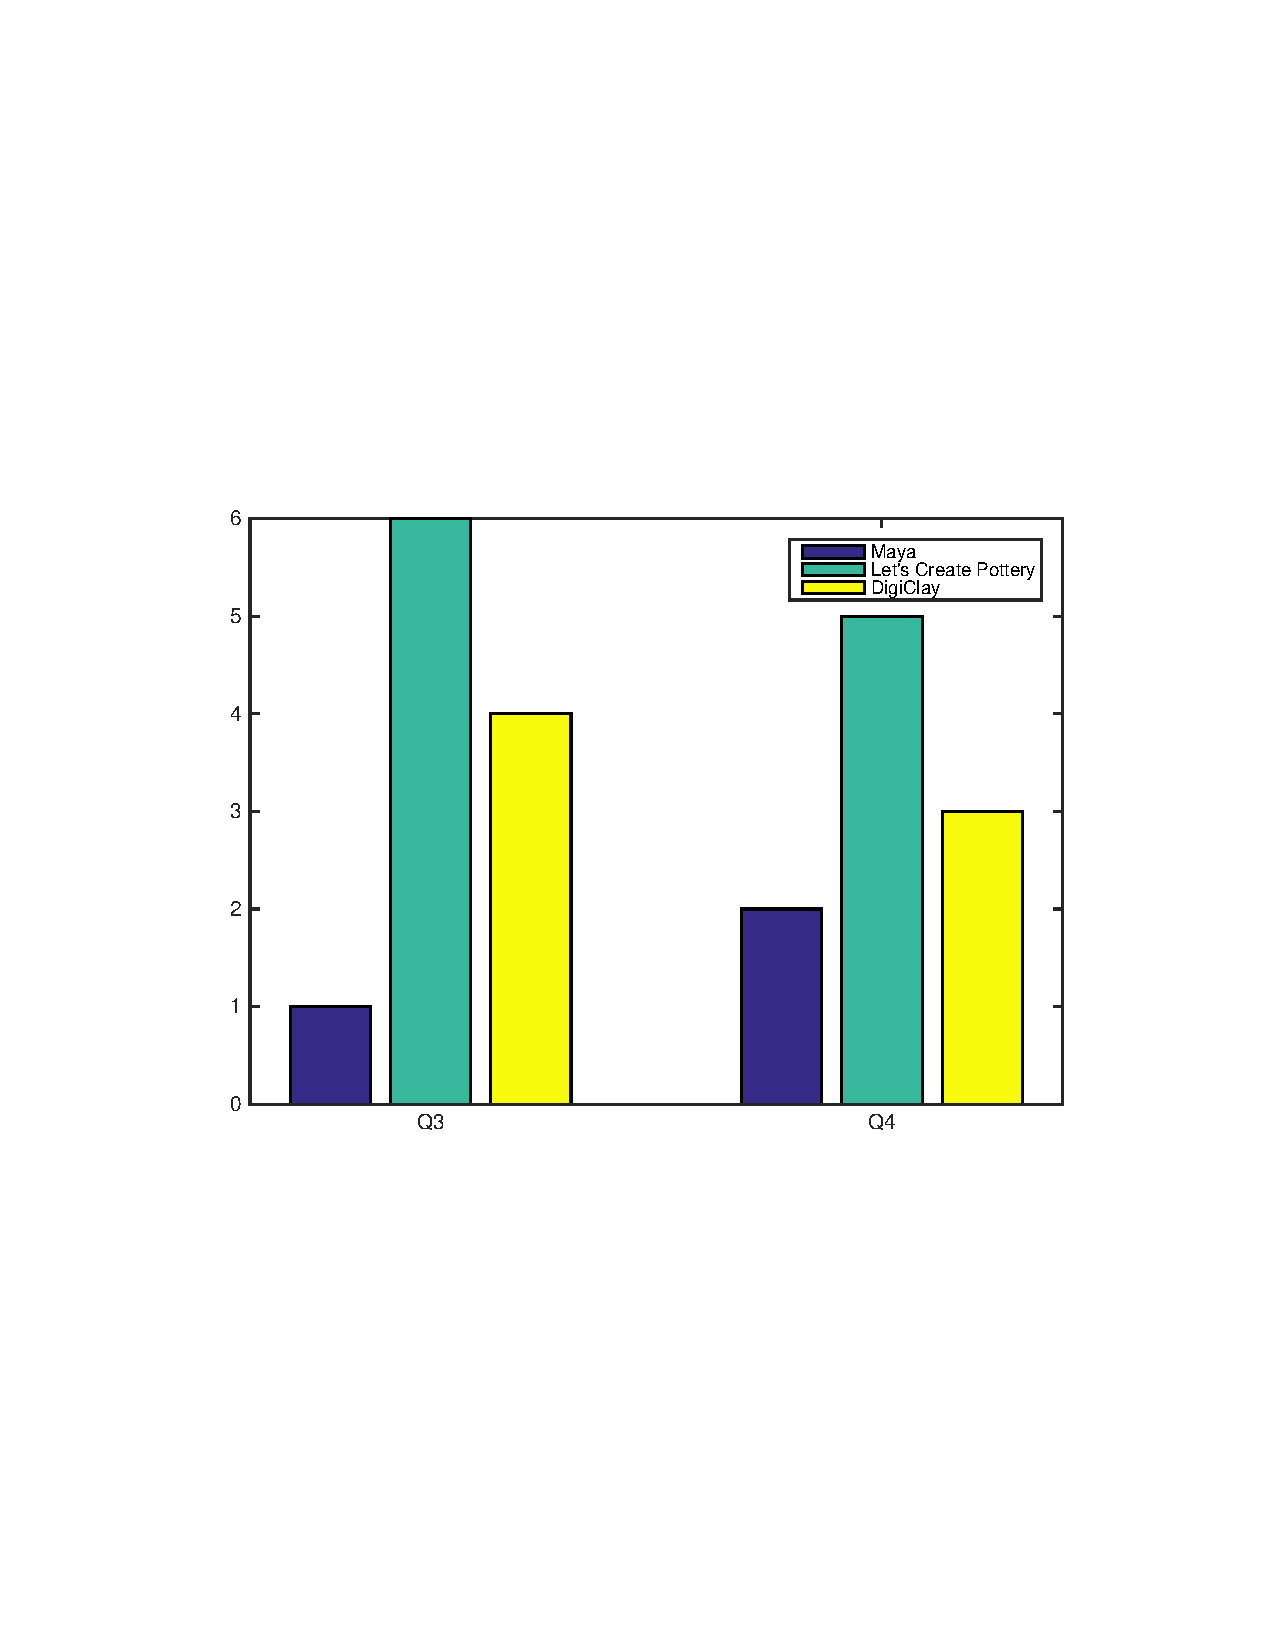
\includegraphics[width=0.75\textwidth]{f8.pdf}
% figure caption is below the figure
\caption{Please write your figure caption here}
\label{fig:1}       % Give a unique label
\end{figure*}

\begin{figure*}
% Use the relevant command to insert your figure file.
% For example, with the graphicx package use
  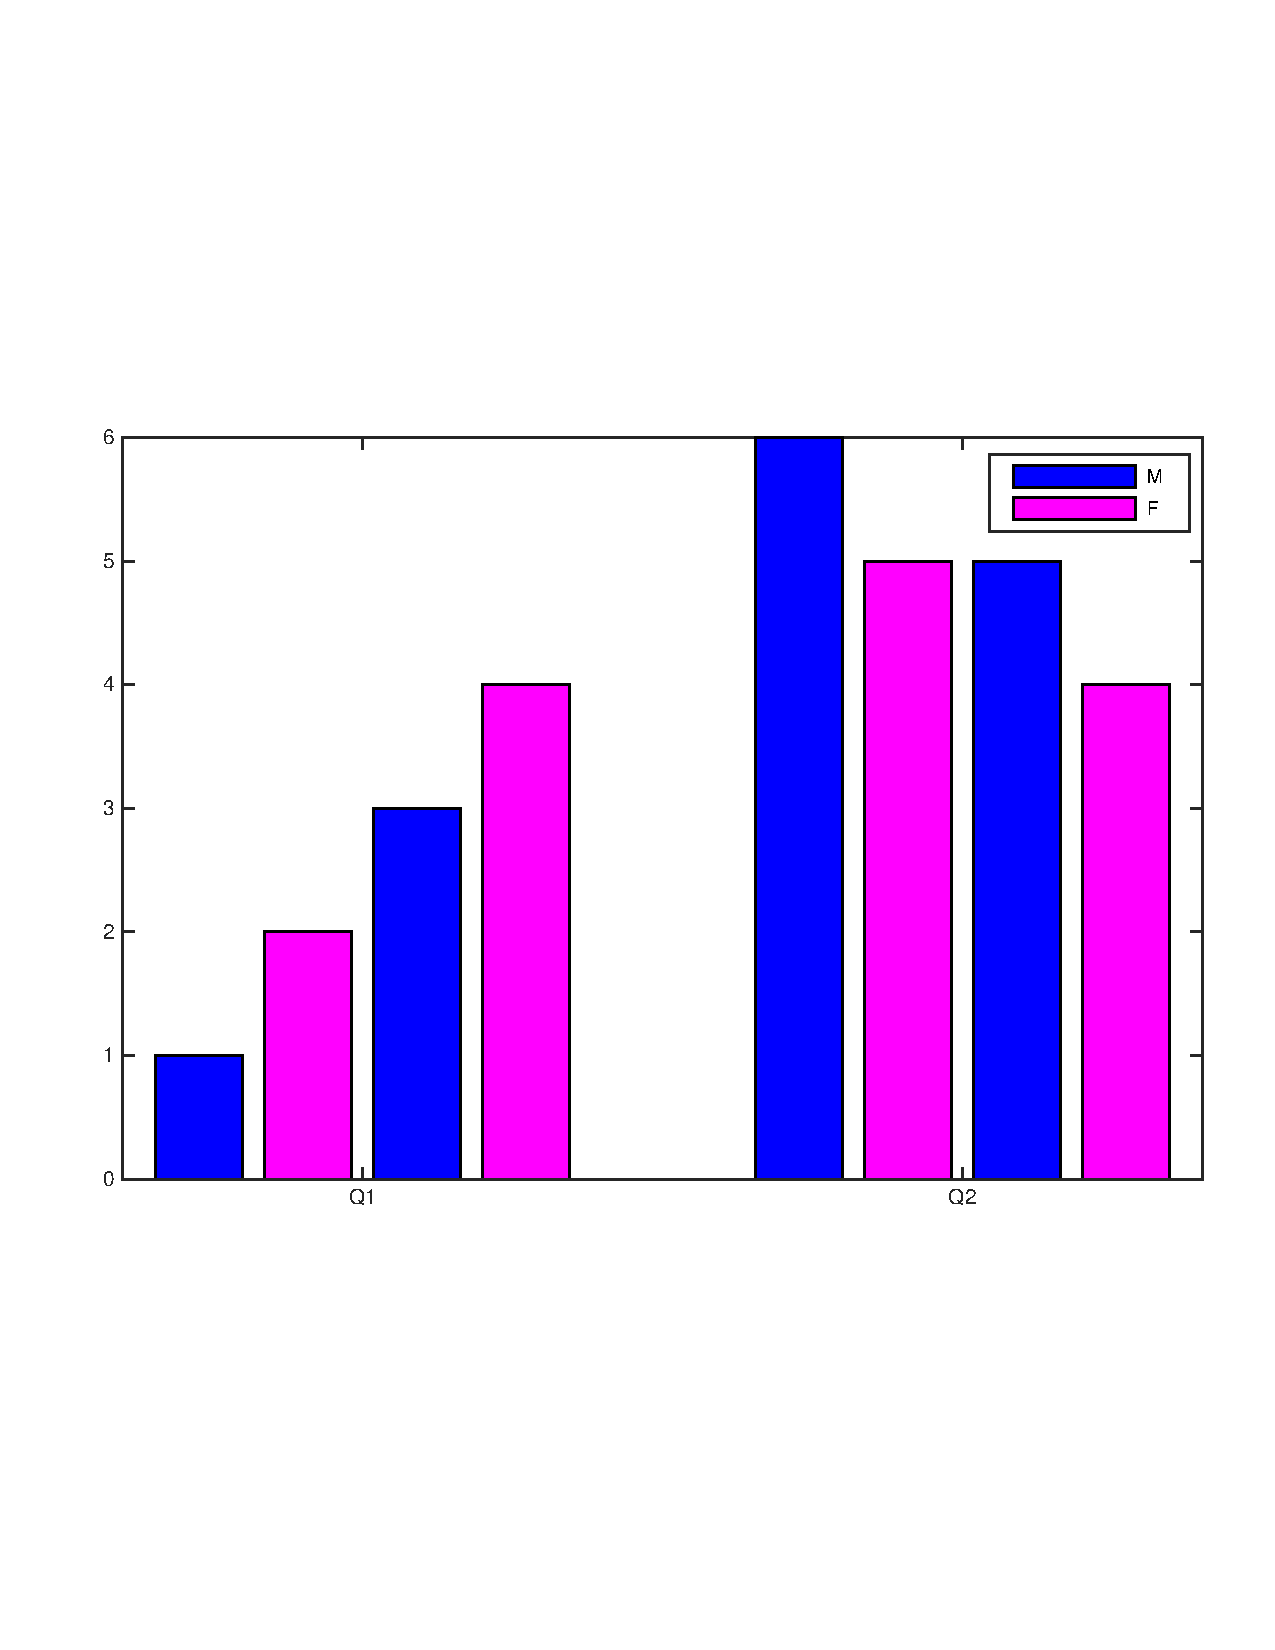
\includegraphics[width=0.75\textwidth]{f9.pdf}
% figure caption is below the figure
\caption{Please write your figure caption here}
\label{fig:1}       % Give a unique label
\end{figure*}

\subsection{User Feedbacks}
\label{sec:6.5}

%[Positive]
We also collected user feedbacks after the subjects had used our system. In summary, subjects gave many positive feedbacks when using our system to design pottery models. They spoke highly of the immersive pottery creation experience with intuitive interaction and haptic feedback that motivated them to design potteries just like working on real clay. In addition, the undo/redo are quite convenient according to the subjects, which enhances the efficiency during the creation process. For those who have no real life pottery creation experience enjoyed our system very much and would like to try real pottery someday. 

%[Suggestions]
During our user study, we found that...
We also asked their suggestions for the future features they wanted to see in DigiClay.
One suggested ...
A few subjects expressed their wishes to add ...
At the end of our user study, many subjects said they would like to try DigiClay one more time.

\section{Limitations}
\label{sec:7}

Our system still has its limitations. First, the physical size of the motion controllers sometimes influence the deformation in bimanual mode, especially when the part of the clay is narrow that two controllers may collide with each other. For example, when subjects working on the neck of clay, it will be difficult to edit with two controllers. This problem can be easily solved by providing user one-hand deformation mode. We plan to use data gloves to avoid these situations in the future.

Second, the potteries designed by our systems lack colors and textures. Although we focus on deformation in our study, several subjects stated that they wish to paint the pottery after designing the shape of the clay. We intend to add new features related to interactive painting on 3D objects.

Another limitation of our system is that it cannot adding handles to the pottery. We will introduce more tools that allow users to modify the topology of the mesh in order to create more personalized pottery works.


\section{Conclusions}
\label{sec:8}

We present PotteryVR, a realtime pottery modeling system in Virtual Reality.
Closely linked to the pottery creation experience real life, our system enables users to manipulate the mesh in realtime with two hands, allowing them creating a variety of pottery models from realistic generated clay meshes.
As an educational tool, PotteryVR can help novice users to learn real life pottery creation process in virtual environment, who can fabricate their works using our system with a 3D printer.
Our results have shown that PotteryVR has relative advantage compared with a traditional desktop 3D tool (Maya) and a mobile app (Let's Create! Pottery).
A possible extension of our system is to support interactive coloring functionalities in the future, which can enhance the artistry of user generated pottery works.


% For one-column wide figures use
\begin{figure}
% Use the relevant command to insert your figure file.
% For example, with the graphicx package use
  
\includegraphics{example.eps}
% figure caption is below the figure
\caption{Please write your figure caption here}
\label{fig:1}       % Give a unique label
\end{figure}
%
% For two-column wide figures use
\begin{figure*}
% Use the relevant command to insert your figure file.
% For example, with the graphicx package use
  
\includegraphics[width=0.75\textwidth]{example.eps}
% figure caption is below the figure
\caption{Please write your figure caption here}
\label{fig:2}       % Give a unique label
\end{figure*}
%


\begin{acknowledgements}
%If you'd like to thank anyone, place your comments here
%and remove the percent signs.
\end{acknowledgements}

% BibTeX users please use one of
%\bibliographystyle{spbasic}      % basic style, author-year citations
\bibliographystyle{spmpsci}      % mathematics and physical sciences
%\bibliographystyle{spphys}       % APS-like style for physics
\bibliography{pottery}   % name your BibTeX data base

% Non-BibTeX users please use
%\begin{thebibliography}{}
%
% and use \bibitem to create references. Consult the Instructions
% for authors for reference list style.
%
%\bibitem{RefJ}
% Format for Journal Reference
%Author, Article title, Journal, Volume, page numbers (year)
% Format for books
%\bibitem{RefB
%Author, Book title, page numbers. Publisher, place (year)
% etc
%\end{thebibliography}

\end{document}
% end of file template.tex

